\section{La technique}

\begin{frame}
  \frametitle{\color{white} test tikz}
  \begin{center}
    \begin{tikzpicture}[scale=1]
      \umlbasicstate[x=0, name=task1, width=8ex]{Tâche 1}
      \umlbasicstate[x=3, name=task2, width=8ex]{Tâche 2}
      \umlbasicstate[x=6, name=task3, width=8ex]{Tâche 3}
      \umlbasicstate[x=0, y=-2.5, name=dev1, width=6ex, fill=green!20]{Dev Princ}
      \umltrans{dev1}{task1}
      \umlbasicstate[x=3, y=-2.5, name=dev2, width=6ex, fill=green!20]{Dev Princ}
      \umltrans{dev2}{task2}
      \umlbasicstate[x=6, y=-2.5, name=dev3, width=6ex, fill=green!20]{Dev Princ}
      \umltrans{dev3}{task3}
      \umlbasicstate[x=1.5, y=-5, name=sup1, width=7ex, fill=red!20]{Dev Support}
      \umltrans{sup1}{dev1}
      \umltrans{sup1}{dev2}
      \umlbasicstate[x=4.5, y=-5, name=sup2, width=7ex, fill=red!20]{Dev Support}
      \umltrans{sup2}{dev2}
      \umltrans{sup2}{dev3}
    \end{tikzpicture}
  \end{center}
\end{frame}

\subsection{Outils de développement}
\begin{frame}
  \frametitle{\color{white} Outils de développement}
  \begin{block}{Langage}
    \begin{itemize}
      \item C++ 11.
      \item Qt 5.
      \hfill
      
\includegraphics[scale=.015]{Qt-logo.png}
    \end{itemize}
  \end{block}
  \begin{block}{Pourquoi le C++ 11 ?}
    \begin{itemize}
      \item Rapidité d'exécution.
      \item Communication simplifiée avec GPG.
      \item Langage natif de Qt.
    \end{itemize}
  \end{block}
  \begin{block}{Pourquoi Qt 5 ?}
    \begin{itemize}
      \item Cadriciel multiplate-forme.
      \item KDE est basé sur ce cadriciel.
    \end{itemize}
  \end{block}
\end{frame}

\subsection{Maquette}
\begin{frame}
  \frametitle{\color{white} Maquette}
  \begin{block}{Livrables}
    \begin{itemize}
      \item Livrable 1 : Gestion des clefs, vue des commandes.
      \item Livrable 2 : Éditeur/opérations cryptographiques.
      \item Livrable 3 : Toile de confiance.
    \end{itemize}
  \end{block}
  \begin{center}
    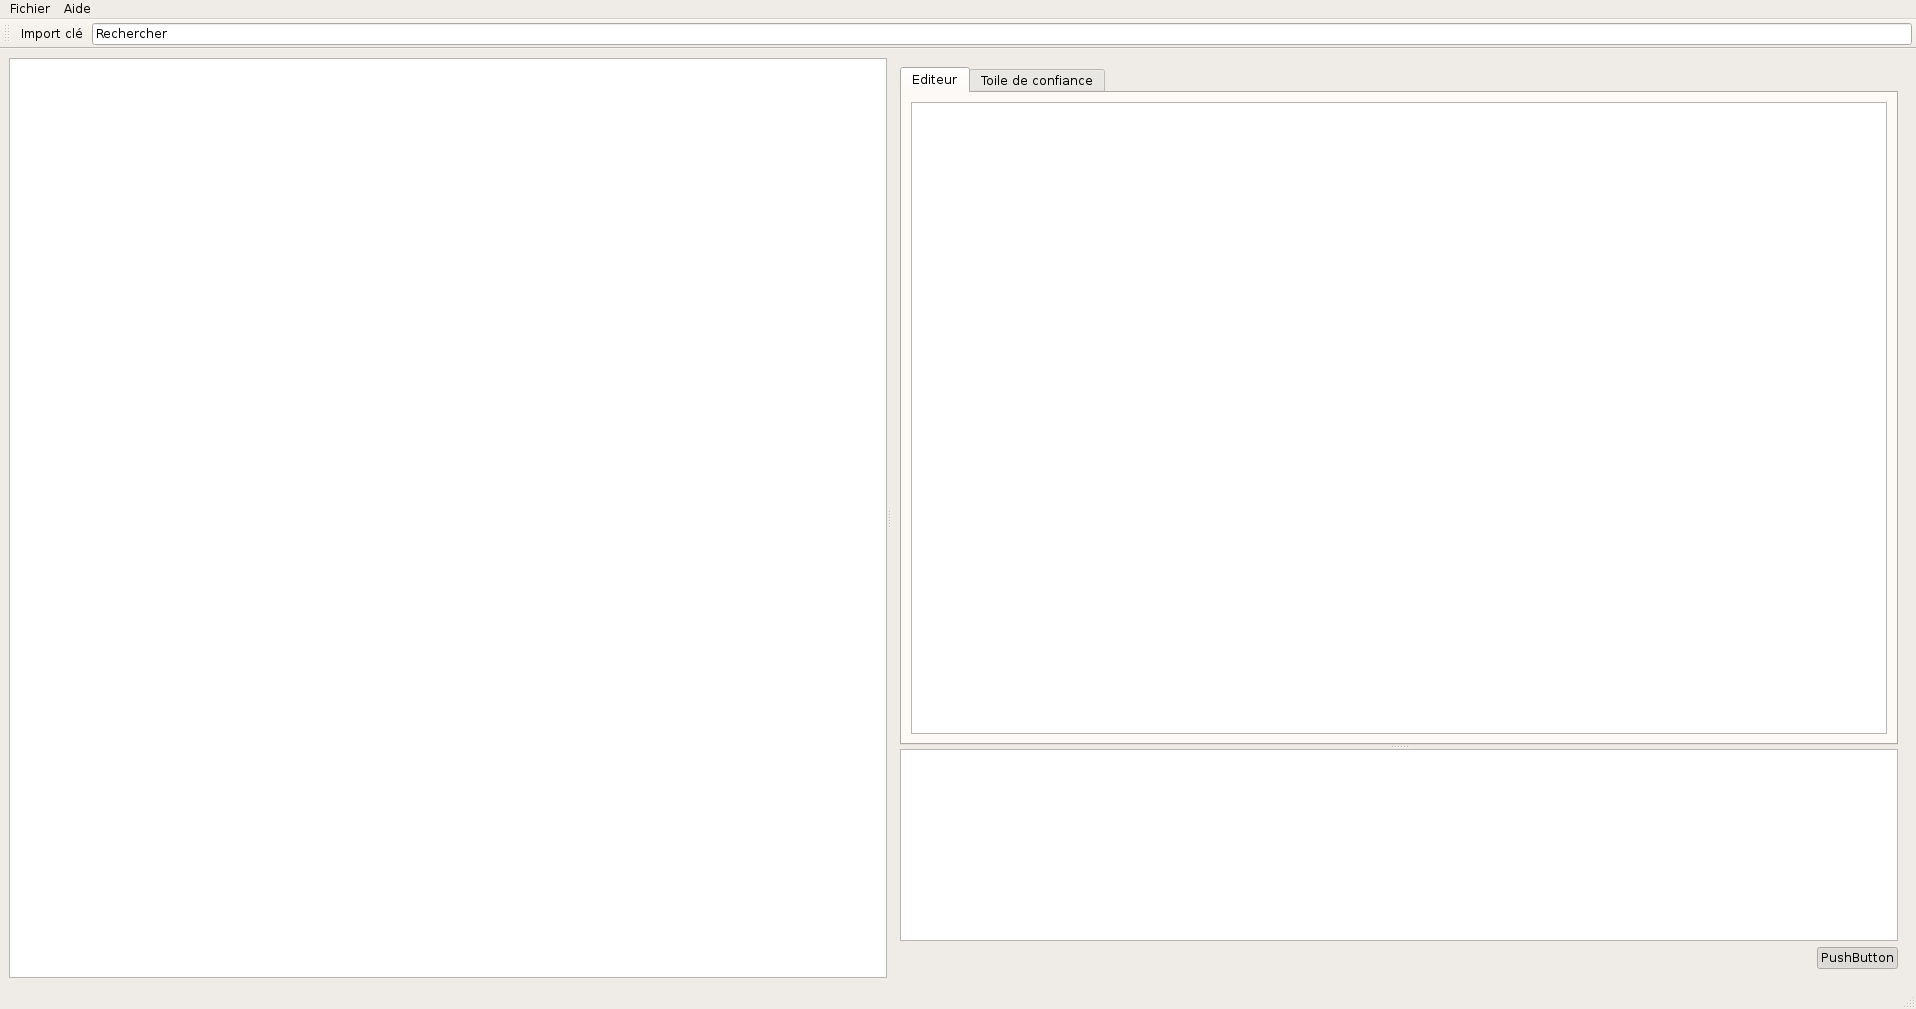
\includegraphics[scale=.14]{maquette.png}
  \end{center}
\end{frame}

\subsection{Procédés de gestion}
\begin{frame}
  \frametitle{\color{white} Procédés de gestion}
  \hfill
  
\includegraphics[scale=.05]{git-logo.png}
  \begin{center}
    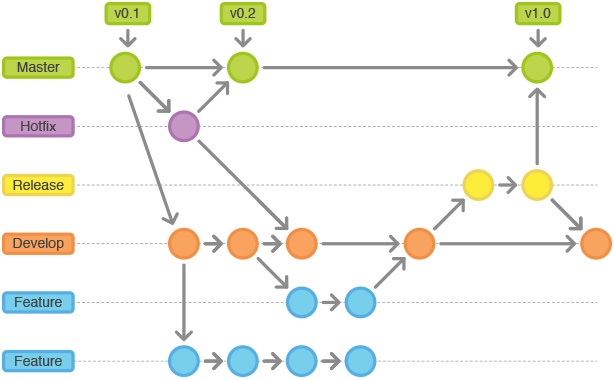
\includegraphics[scale=.45]{git_workflow}
  \end{center}
\end{frame}